\documentclass{article}

%\usepackage{psfig}

\setlength{\evensidemargin}{0in} \setlength{\oddsidemargin}{0in}
\setlength{\textwidth}{6.7in} \setlength{\topmargin}{-1.1in}
\setlength{\textheight}{10.5in}


\usepackage{amssymb, amsthm, amstext, amsxtra, amsmath, amsfonts, amscd }
\usepackage{graphicx, epsfig}
\usepackage{comment}
\usepackage{color}
\usepackage{cleveref}
\usepackage{listings, tikz}


\def\E{\mathbb{E}}
\def\pr{\mathbb{P}}

\renewcommand\baselinestretch{1.2}

\DeclareMathOperator{\sign}{sign}
\DeclareMathOperator{\supp}{supp}

\DeclareMathOperator{\Cov}{Cov}
\DeclareMathOperator{\Var}{Var}
\DeclareMathOperator{\corr}{corr}

\author{Salvador Garcia, s1655274}

\date{28 Marzo 2017}


\title{Assignment 1: Modelling the skills of Go players}

\begin{document}
\maketitle
\section{Question 3}

\subsection*{b)}
\begin{figure}[ht!]
    \centering
    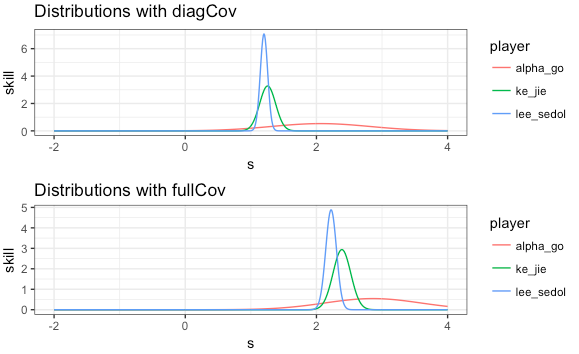
\includegraphics[scale=.7]{im1.png}
    \caption{Posterior distributions with full and diag covariance matrix}
    \label{fig:fig1}
\end{figure}
\begin{lstlisting}
library(tidyverse)
library(R.matlab)

diagCov <- readMat("diag_covar.mat")
fullCov <- readMat("full_covar.mat")

attach(diagCov) #---------------------------
s = seq(-2,4, by = .01)
alpha_go <- dnorm(s, approx.mean[alpha.go.id], sqrt(approx.covar[alpha.go.id]))
ke_jie <- dnorm(s, approx.mean[ke.jie.id], sqrt(approx.covar[ke.jie.id]))
lee_sedol <- dnorm(s, approx.mean[lee.sedol.id], sqrt(approx.covar[lee.sedol.id]))

diagcov_df <- data.frame(s, alpha_go, ke_jie, lee_sedol) %>% 
  gather(player, skill, -s)
  


  
p1 <- diagcov_df %>% 
  ggplot(aes(x = s, y = skill, group = player, color = player))+
  geom_line() +
  labs(title = "Distributions with diagCov")+
  theme_bw()
detach(diagCov) 

attach(fullCov) #---------------------------
s = seq(-2,4, by = .01)
alpha_go <- dnorm(s, approx.mean[alpha.go.id], sqrt(approx.covar[alpha.go.id,alpha.go.id]))
ke_jie <- dnorm(s, approx.mean[ke.jie.id], sqrt(approx.covar[ke.jie.id, ke.jie.id]))
lee_sedol <- dnorm(s, approx.mean[lee.sedol.id], sqrt(approx.covar[lee.sedol.id, lee.sedol.id]))

fullcov_df <- data.frame(s, alpha_go, ke_jie, lee_sedol) %>% 
  gather(player, skill, -s)

p2 <- fullcov_df %>% 
  ggplot(aes(x = s, y = skill, group = player, color = player))+
  geom_line() +
  labs(title = "Distributions with fullCov")+
  theme_bw()
detach(fullCov) 
  
grid.arrange(p1, p2)
\end{lstlisting}


\subsection*{c)}

\begin{lstlisting}

attach(diagCov) #---------------------------
x_k = rep(0, n.players)
x_k[alpha.go.id] = 1/sqrt(2)
x_k[ke.jie.id] = -1/sqrt(2)

val_diag <- (approx.mean%*%as.matrix(x_k))/
  sqrt(t(as.matrix(x_k))%*%diag(c(approx.covar))%*%as.matrix(x_k)+1)
pnorm(val_diag)
detach(diagCov) 

attach(fullCov) #---------------------------
# vector x_k
x_k = rep(0, n.players)
x_k[alpha.go.id] = 1/sqrt(2)
x_k[ke.jie.id] = -1/sqrt(2)

val_ful <- (approx.mean%*%as.matrix(x_k))/
  sqrt(t(as.matrix(x_k))%*%approx.covar%*%as.matrix(x_k)+1)
pnorm(val_ful)
detach(fullCov) 
\end{lstlisting}


\end{document}
